\subsection{斜线在平面上的射影,直线和平面所成的角}\label{subsec:1-10}

自一点向平面引垂线,垂足叫做\zhongdian{这点在这个平面上的射影}。
这个点与垂足间的线段叫做\zhongdian{这点到这个平面的垂线段}。

一条直线和一个平面相交,但不和这个平面垂直,这条直线叫做\zhongdian{这个平面的斜线},
斜线和平面的交点叫做\zhongdian{斜足}。
斜线上一点与斜足间的线段叫做\zhongdian{这点到这个平面的斜线段}。

过斜线上的一点向平面引垂线,过垂足和斜足的直线叫做\zhongdian{斜线在这个平面上的射影},
垂足与斜足间的线段叫做这点到平面的\zhongdian{斜线段在这个平面上的射影}。
斜线上任意一点在平面上的射影,一定在斜线的射影上。

如图 \ref{fig:ltjh-1-30},对于平面 $\alpha$,直线 $AB$ 是垂线,垂足 $B$ 是点 $A$ 的射影;
直线 $AC$ 是斜线,$C$ 是斜足,直线 $BC$ 是斜线 $AC$ 的射影;
线段 $AB$ 是垂线段,线段 $AC$ 是斜线段,线段 $BC$ 是斜线段 $AC$ 的射影。

\begin{figure}[htbp]
    \centering
    \begin{minipage}[b]{7cm}
        \centering
        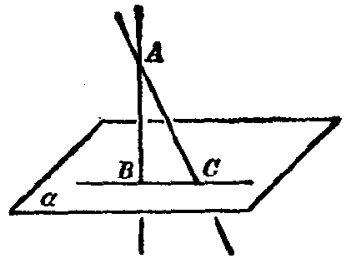
\includegraphics[width=4cm]{../pic/ltjh-ch1-30.png}
        \caption{}\label{fig:ltjh-1-30}
    \end{minipage}
    \qquad
    \begin{minipage}[b]{7cm}
        \centering
        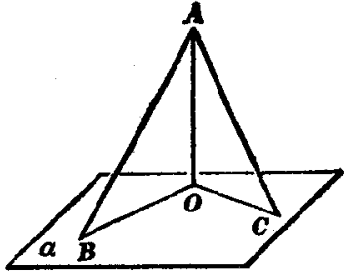
\includegraphics[width=4cm]{../pic/ltjh-ch1-31.png}
        \caption{}\label{fig:ltjh-1-31}
    \end{minipage}
\end{figure}

根据直角三角形性质,我们很容易得到:

\begin{dingli}[定理][dl:pmwyd-cxd-xxd]
    从平面外一点向这个平面所引的垂线段和斜线段中,

    (1)射影相等的两条斜线段相等,射影较长的斜线段也较长;

    (2)相等的斜线段的射影相等,较长的斜线段的射影也较长;

    (3)垂线段比任何一条斜线段都短。
\end{dingli}

如图 \ref{fig:ltjh-1-31},$AO$ 是平面 $\alpha$ 的垂线段,$AB$、$AC$ 是平面 $\alpha$ 的斜线段,
$OB$、$OC$ 分别是 $AB$、$AC$ 在平面 $\alpha$ 上的射影。这时有:

(1) \begin{zmtblr}[t]{}
    $OB = OC  \tuichu  AB = AC$, \\
    $OB > OC  \tuichu  AB > AC$;
\end{zmtblr}

(2)\begin{zmtblr}[t]{}
    $AB = AC  \tuichu  OB = OC$, \\
    $AB > AC  \tuichu  OB > OC$;
\end{zmtblr}

(3)$AO < AB$, $AO < AC$。

下面研究直线与平面所成的角。 例如,发射炮弹时,炮筒和地平面所成的角。

平面的一条斜线和它在平面上的射影所成的锐角,叫做\zhongdian{这条直线和这个平面所成的角}(图 \ref{fig:ltjh-1-32})。

一条直线垂直于平面,我们说它们\zhongdian{所成的角是直角};
一条直线和平面平行,或在平面内,我们说它们\zhongdian{所成的角是 $\bm{0^\circ}$的角}。

可以证明,\zhongdian{斜线和平面所成的角,是这条斜线和平面内经过斜足的直线所成的一切角中最小的角。}

如图 \ref{fig:ltjh-1-32}, $l$ 是平面 $\alpha$ 的斜线,$A$ 是 $l$ 上任意一点,
$AB$ 是平面 $\alpha$ 的垂线,$B$ 是垂足,所以直线 $OB$ 是斜线 $l$ 的射影,
$\angle \theta$ 是斜线 $l$ 与平面 $\alpha$ 所成的角。
设 $OD$ 是平面 $\alpha$ 内与 $OB$ 不同的任意一条直线,$AC$ 垂直于 $OD$,垂足为 $C$。
因为垂线段 $AB$ 小于斜线段 $AC$,所以在有公共斜边 $OA$ 的直角三角形 $OAB$、$OAC$ 中,
$\sin\theta < \sin AOC$。 因此 $\angle \theta < \angle AOC$。

\begin{figure}[htbp]
    \centering
    \begin{minipage}[b]{7cm}
        \centering
        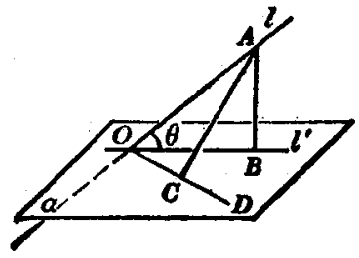
\includegraphics[width=5cm]{../pic/ltjh-ch1-32.png}
        \caption{}\label{fig:ltjh-1-32}
    \end{minipage}
    \qquad
    \begin{minipage}[b]{7cm}
        \centering
        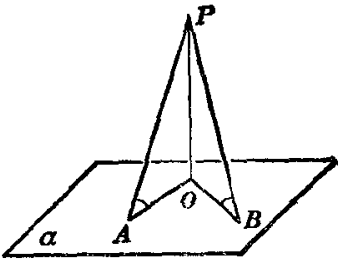
\includegraphics[width=5cm]{../pic/ltjh-ch1-33.png}
        \caption{}\label{fig:ltjh-1-33}
    \end{minipage}
\end{figure}

\liti[0] 两条斜线段 $PA$、$PB$ 和平面 $\alpha$ 所成的角相等的充要条件是 $PA = PB$。

已知:$PA$、$PB$ 是平面 $\alpha$ 的两条斜线段,$PO$ 是垂线段(图 \ref{fig:ltjh-1-33})。

求证:$\angle PAO = \angle PBO  \dengjiayu  PA = PB$。

\zhengming (1)先证 $\angle PAO = \angle PBO  \tuichu  PA = PB$。

\jiange
$\left.\begin{aligned}
    \left.\begin{aligned}
        PO \perp \alpha \\
        OA \subset \alpha \\
        OB \subset \alpha
    \end{aligned}\right\}  \tuichu  \left\{\begin{aligned}
        PO \perp OA \\
        PO \perp OB
    \end{aligned}\right. \\
    PO = PO \\
    \angle PAO = \angle PBO
\end{aligned}\right\}  \tuichu  Rt \triangle PAO \quandeng Rt \triangle PBO  \tuichu  PA = PB \juhao$

\jiange
(2)再证 $PA = PB  \tuichu  \angle PAO = \angle PBO$。

类似地,由 $PA = PB$ 可证 $Rt \triangle PAO \quandeng Rt \triangle PBO$,于是得
$$\angle PAO = \angle PBO \juhao$$

$\therefore$ \quad $\angle PAO = \angle PBO  \dengjiayu  PA = PB$。


\begin{lianxi}

\xiaoti{将本节的\hyperref[dl:pmwyd-cxd-xxd]{定理}中的(1)、(2)改为用充要条件来叙述。}

\xiaoti{已知斜线段的长是它在平面 $\alpha$上射影的 2 倍,求斜线和平面 $\alpha$ 所成的角。}

\xiaoti{两条直线和一个平面所成的角相等,它们平行吗?}

\end{lianxi}
